\section{Related Work}
\label{sec:Related Work}

This paper builds on several recent results in the design and fabrication of soft robots; see \citep{lipson2013challenges}, \citep{rus2014soft}, \citep{marchese2014thesis} for detailed reviews.

\subsection{Actuation}
\label{subsec:RW Actuation}
There are various approaches to actuating the body of a soft robot.
One distinguishing feature of many soft robots is that actuators and/or power transmission systems are integrated within and distributed throughout the body.
In the following we review four common actuator types, and these are also depicted in Figure~\ref{fig:RW actuation}.
\begin{figure}
  \centering
  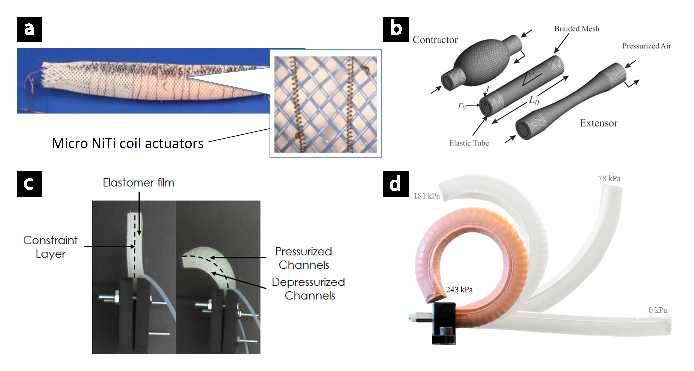
\includegraphics[width=3in]{figures/relatedwork/actuation.eps}
  \caption[Common actuation approaches for soft robots.]{Common actuation approaches for soft robots. (\textbf{a}) Shape Memory Alloy (SMA) actuators \citep{seok2010peristaltic}, (\textbf{b}) Pneumatic Artificial Muscle (PAM) actuators \citep{mcmahan2006field}, (\textbf{c}) Fluidic Elastomer Actuators (FEAs) \citep{onal2011soft}, and (\textbf{d}) Fiber reinforced FEAs \citep{galloway2013mechanically}.}\label{fig:RW actuation}
\end{figure}

\subsubsection{Shape Memory Alloy Actuators}
\label{subsubsec:RW SMA}
\hl{The basic operating principle behind Shape Memory Alloy (SMA) technology is that nickel titanium (NiTi) wire contracts under joule heating.
This heating is typically produced by passing electrical current through the wire.
The contracting wire can be used as an agonist actuator, similar to the way one's bicep pulls the forearm towards the body.
\mbox{\citet{kim2009micro}} model, design, and fabricate these actuators and show their viability in soft robot applications.
Additionally, the elastomer-based bio-inspired octopus arms developed in \mbox{\citet{laschi2012soft}} and \mbox{\citet{cianchetti2014bioinspired}} use SMA actuation to emulate a muscular hydrostat.
Further, \mbox{\citet{seok2010peristaltic}} use SMA spring actuators to generate peristaltic locomotion in a worm-like robot (see Fig.~\mbox{\ref{fig:RW actuation}}a), \mbox{\citet{koh2013omega}} develop SMA coil-spring actuators to generate two-anchor crawling in an inchworm-like robot, and \mbox{\citet{umedachi2013highly}} use SMA actuators to produce both crawling and inching in 3D printed soft robot.}


\subsubsection{Cable Actuators}
\label{subsubsec:RW Cables}
Originally, many hard hyper redundant and hard continuum robots \citep{cieslak1999elephant, buckingham2002snake, gravagne2002uniform, hannan2003kinematics, mcmahan2005design, camarillo2009configuration} used an array of servomotors or linear actuators to pull cables that move rigid connecting plates located between body segments.
Some softer robots have adopted a similar actuation scheme consisting of tendons pulling rigid fixtures embedded within an elastomer body.
\hl{For example, the soft-bodied fish developed by \mbox{\citet{youcef2006design}}, the soft octopus-inspired arms developed in \mbox{\citet{calisti2010study}} and \mbox{\citet{calisti2011octopus}}, as well as the soft arm developed by \mbox{\citet{wang2013visual}} use this actuation approach.}

\subsubsection{Pneumatic Artificial Muscles}
\label{subsubsec:RW PMA}
Another common actuation scheme for soft robots involves distributed Pneumatic Artificial Muscle (PAM) actuators, also known as McKibben actuators and shown in Figure~\ref{fig:RW actuation}b.
A PAM is fundamentally composed of an inflatable elastic tube surrounded by a braided mesh.
Depending on the weave pattern of the braided mesh, the actuator can be designed to contract or extend under input pressure.
Typically, these actuators are operated with driving pressures between 50 to 100 ~psi.
\hl{These actuators have been used and studied extensively in \mbox{\citet{chou1996measurement, tondu2000modeling}} \mbox{\citet{caldwell2000bio, daerden2002pneumatic}} and \mbox{\citet{reynolds2003modeling}}.}
Notable semi-soft robots using PAMs include \citet{mcmahan2006field, pritts2004design} and \citet{kang2013design}.

\subsubsection{Fluidic Elastomer Actuators}
\label{subsubsec:RW FEA}
A softer alternative is the Fluidic Elastomer Actuator (FEA), which is used predominantly throughout this paper (see Fig.~\ref{fig:RW actuation}c).
The FEA is an actuator composed of low durometer rubber and driven by relatively low-pressure fluid in the range of 3 to 8~psi.
\hl{Although many motion primitives are achievable with a FEA (e.g., extending, contracting, twisting, and bending) in this work we primarily focus on actuators designed for bending.}
Its basic structure consists of two soft elastomer layers separated by a flexible, but relatively inextensible constraint.
\hl{The inextensible constraint is typically created using cloth, paper, plastics, and even stiffer rubbers.}
Each of these elastomer layers contains embedded fluidic channels.
By pressurizing the fluid entrapped in these channels, stress is induced within the elastic material producing localized strain. This strain in combination with the relative in-extensibility of the constraint produces body segment bending.
FEAs can be powered pneumatically or hydraulically.

\hl{As the review by \mbox{\citet{rus2014soft}} discusses,} perhaps the earliest application of pneumatically actuated elastomer bending segments to robotics was by \citet{suzumori1992applying}.
Here fiber-reinforced Flexible Microactuators (FMAs) were developed and shown to be viable in a manipulator and multi-fingered hand.
\hl{Recently, these concepts have been extended and developed into the FEA and used to build a variety of soft mechanisms \mbox{\citep{shepherd2011multigait, ilievski2011soft, morin2012camouflage}}
\mbox{\citep{martinez2013robotic}}
and soft robotic systems
\mbox{\citep{onal2011soft, marchese2011soft, onal2013autonomous}}
\mbox{\citep{marchese2014autonomous, marchese2014design, marchese2014whole}}
\mbox{\citep{katzschmann2014hydraulic, katzschmann2015autonomous}}
\mbox{\citep{tolley2014untethered, tolley2014resilient}} \mbox{\citep{marchese2015design}}
\mbox{\citep{marchese2015control, marchese2015dynamics}}.}
Furthermore, \citet{polygerinos2013towards} and \citet{mosadegh2014pneumatic} have investigated more elaborate channel designs in order to reduce elastomer strain on the outer layer of the actuator, allowing for higher bending curvatures.
\hl{Additionally, \mbox{\citet{cianchetti2014soft}} develop a fluid actuated bending arm with a jamming \mbox{\citep{brown2010universal, liu1998nonlinear}} spine.}

There are also less flexible, fiber-reinforced FEAs (see Fig.~\ref{fig:RW actuation}d) that occupy the soft actuator space between purely elastomer FEAs and PAMs.
While these actuators have to operate with comparably higher driving pressures between 25 and 35~psi, they can accordingly apply higher forces which is advantageous for certain applications.
There are several notable examples of fiber-reinforced FEAs in the literature \citet{suzumori1992applying, suzumori2007bending, bishop2012design, galloway2013mechanically, deimel2013compliant, deimel2014novel} and \citet{park2014design}.

\subsection{Design Tools}
\label{subsec:RW Design Tools}
Design tools for soft robots are limited with respect to the availability of design tools for more traditional rigid-body robots.
\citet{suzumori2007bending} use Finite Element Modeling (FEM) to analyze the bending of fiber re-inforced pneumatic tube-like actuators.
Specifically, hyper-elastic material models are used to capture the nonlinear material properties of rubber, line elements are used to represent radial in-extensibility constraints due to fiber reinforcement, and the simulation is performed using the software MARC.
Outside of this example, the community has generally found that iterative nonlinear finite element solvers are limited to small deformations and of limited use when modeling very soft nonlinear materials \citep{lipson2014challenges}.
VoxCAD and the Voxelyze physics engine, as used in \citet{cheney2013unshackling} and \citet{lehman2011evolving} and reviewed by \citet{lipson2014challenges}, are simulation tools for very soft nonlinear materials.
These tools use the concept of nonlinear relaxation to effectively perform physically correct particle-based material simulation.
They have the advantage of allowing the user to individually set the local material properties of each particle.
The disadvantage is that many physical parameters of active and passive material types must be experimentally derived.

\subsection{Fabrication}
\label{subsec:RW Fabrication}
\citet{cho2009review} review several manufacturing processes for soft biomimetic robots.
The vast majority of soft elastomer robots rely on the processes of soft lithography \citep{xia1998soft} and/or shape deposition manufacturing \citep{cham2002fast}.
Specifically, for soft fluidic elastomer robots this fabrication process generally consists of three steps as shown in Figure~\ref{fig:RW fabrication}: (1) Two elastomer layers are molded through a casting process using pourable silicone rubber. The mold used for the outer layer contains a model of the desired channel structure. When cast, the outer layer contains a negative of this channel structure. The mold used for the constraint layer may contain fiber, paper, or a plastic film to produce the the in-extensibility property required for actuation. When the elastomer is poured, this material is effectively embedded within the constraint layer.
(2) The two layers are cured, removed from their molds, and their joining faces are dipped in a thin layer of uncured elastomer.
(3) Lastly, the two layers are joined and cured together.
The primary limitation of this soft lithography fabrication process is that it is fundamentally 2.5D, meaning that the robots are largely constrained to a planar morphology.
This process limits a soft robot's ability to achieve amorphous, 3D forms.
Additionally, \citet{umedachi2013highly} provide the first SMA actuated soft robot fabricated using 3D printing.
However, although 3D printing allows printing flexible materials in amorphous forms, these materials are relatively brittle with respect to casted rubbers and are therefore not well-suited for FEAs, which rely on pressurization of the rubber.
\begin{figure}
  \centering
  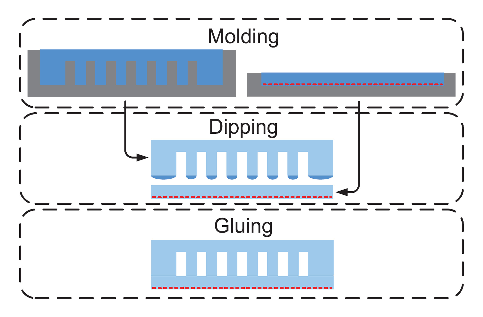
\includegraphics[width=3in]{figures/relatedwork/fabrication.eps}
  \caption[Soft lithography fabrication process.]{Soft lithography fabrication process for soft fluidic elastomer robots. Reproduced with permission from \citet{onal2012modular}.}\label{fig:RW fabrication}
\end{figure}

\subsection{Soft Locomotory Robots}
\label{subsec:RW Land}
In the past years, soft roboticists have made many notable low durometer rubber robots intended for land and water locomotion.
For example, rolling belts have been produced by \citet{correll2010soft} and \citet{marchese2011soft}.
\citet{trimmer2006caterpillar} and \citet{umedachi2013highly} emulated the peristaltic locomotion of caterpillars. \citet{shepherd2011multigait} developed a multi-gait walking robot, and \citet{shepherd2013using} developed a jumping robot powered by combustion.
However, a limitation of the aforementioned locomotory robots is that they require an electrical and/or pneumatic tether.
Soft actuation systems, especially fluidic actuation systems, typically require significant supporting hardware and often limit soft locomotory robots from being self-contained.
That said, there are a few examples of untethered soft robots:
\citet{onal2011soft} created a rolling robot, \citet{onal2013autonomous} emulated the serpentine locomotion of snakes, and \cite{tolley2014resilient} developed a quadrupedal walking robot; these are all soft-bodied fluidic elastomer systems.
\citet{seok2010peristaltic} realize peristaltic locomotion with a self-contained SMA-based inchworm.
However, a limitation of all these untethered soft platforms is that performance is severely limited with respect to their rigid-bodied counterparts, and this limitation is due to the constraints imposed by bringing onboard all supporting hardware.
More specifically, they all exhibit locomotory speeds of between 0.008 and 0.07 body lengths per second.
Recently, \citet{marchese2014autonomous} developed an autonomous soft robotic fish that can perform escape maneuvers with speeds up to 0.4 body lengths per second. \citet{katzschmann2014hydraulic} presented a soft fish that can swim in 3D for prolonged periods of time and powers its FEA tail hydraulically.

\subsection[Soft Continuum Manipulators]{Soft Continuum Manipulators\footnote{\hl{This subsection also appears in the author's related work} \citet{marchese2015design}.}}
Recently, continuum manipulators composed from soft elastic material have been developed.
These soft rubber manipulators can be categorized under two primary morphologies.
The first morphology-type are tendon driven manipulators consisting of variable length tendons, typically cables or shape memory alloy wire (see Section \ref{subsubsec:RW Tendons}), embedded within and anchored to portions of a soft silicone rubber arm.
For example, previous work on soft bio-inspired octopus-like arms developed by \citet{calisti2010study} used tendons and demonstrated capabilities like grasping and locomotion \citep{laschi2012soft, calisti2011octopus}.
Also, \citet{wang2013visual} developed a cable driven soft rubber arm consisting of one large actuated segment that bends bi-directionally.
Lastly, \citet{mcevoy14shape} and \citet{mcevoy2014thermoplastic} used a programmable stiffness spine in conjunction with tendons to achieve shape change in a soft rubber arm.
The second morphology uses fluidic elastomer actuators (see Section~\ref{subsubsec:RW FEA}) distributed among the manipulator's soft body segments.
The primary advantages of using fluidic actuation for soft continuum manipulators is that this energy transmission system: (i) can be lightweight making for easy integration into distal locations of the body, (ii) conforms to the time varying shape of the manipulator, and (iii) does not require rigid components to implement.
There are several examples of soft fluidic grippers described in recent literature.
\citet{deimel2013compliant} developed a pneumatically actuated three-fingered hand made of fiber reinforced silicone that is mounted to a hard industrial robot and capable of robust grasping.
More recently, they have used similar fiber reinforced actuation technology to develop an anthropomorphic soft pneumatic hand capable of dexterous grasps \citep{deimel2014novel}.
Additionally, we have previously shown planar manipulation is possible with an entirely soft robot. That is, a six-segment planar fluidic elastomer robot can be precisely positioned using a closed-loop kinematic controller \citep{marchese2014design, marchese2014whole, katzschmann2015autonomous}.
\citet{ilievski2011soft} created a pneumatic starfish-like gripper composed of FEAs and demonstrated it grasping an egg.
\citet{Stokes2014hybrid} used an FEA-based elastomer quadrupedal robot to grasp objects in a hard-soft hybrid robotic platform.
A puncture resistant soft pneumatic gripper is developed in \citet{shepherd2013soft}.
An alternative to positive pressure actuated soft grippers is the robotic gripper based on the jamming of granular material developed in \citet{brown2010universal}.
Another relevant piece of work is the manually operated 3D elastomer tentacles developed by \citet{martinez2013robotic} containing 9 pneumatic crescent-shaped channels embedded within 3 body segments.

